\documentclass[11pt]{article}
\usepackage[margin=1in]{geometry}
\usepackage{graphicx}
\usepackage{booktabs}
\usepackage{array}
\setlength{\parskip}{0.45em}
\setlength{\parindent}{0pt}

\newcommand{\fixedfig}[2]{%
  \par\vspace{0.4em}%
  \noindent\begin{minipage}{\textwidth}%
  \centering
  #1\par\vspace{0.4em}%
  {\small #2}%
  \end{minipage}%
  \par\vspace{0.9em}%
}

\title{ECS 174 Homework 2\\Training a DCGAN on CelebA}
\author{Sol Abrian}
\date{}

\begin{document}
\maketitle

Three experiments follow the PyTorch DCGAN faces tutorial. Images are resized to \(64\times 64\) and scaled to the range \(-1\) to \(1\). Training uses Adam with learning rate \(0.0002\), \(\beta_1=0.5\), batch size 128, and binary cross entropy, for 5 epochs. CelebA has 202,599 images. On this CPU one full pass takes a little over 3 hours, so each experiment uses the first 12,800 images (100 batches). The generator is shown on one fixed noise batch after every epoch.

\section{Experiment 1: baseline DCGAN}

The generator and discriminator are the tutorial networks. The discriminator is updated once per batch, then the generator is updated once on that same batch.

\begin{center}
\small
\begin{tabular}{@{}cccccc@{}}
\toprule
Epoch & Batch & Loss\(_D\) & Loss\(_G\) & \(D(x)\) & \(D(G(z))\) \\
\midrule
1 & 0 & 1.8134 & 2.1164 & 0.3093 & 0.3012 / 0.1568 \\
1 & 50 & 0.1597 & 16.2452 & 0.9245 & 0.0001 / 0.0000 \\
2 & 0 & 0.0039 & 41.3520 & 0.9964 & 0.0000 / 0.0000 \\
2 & 50 & 0.0047 & 40.7841 & 0.9956 & 0.0000 / 0.0000 \\
3 & 0 & 0.0012 & 40.5421 & 0.9989 & 0.0000 / 0.0000 \\
3 & 50 & 0.0005 & 40.3305 & 0.9995 & 0.0000 / 0.0000 \\
4 & 0 & 0.0001 & 40.3957 & 0.9999 & 0.0000 / 0.0000 \\
4 & 50 & 0.0001 & 40.1920 & 0.9999 & 0.0000 / 0.0000 \\
5 & 0 & 0.0002 & 39.9765 & 0.9998 & 0.0000 / 0.0000 \\
5 & 50 & 0.0000 & 39.1484 & 1.0000 & 0.0000 / 0.0000 \\
\bottomrule
\end{tabular}
\end{center}

By the end of epoch 1 the discriminator is already sure: \(D(x)\) is near 1 and \(D(G(z))\) is 0. The generator loss then sits near 40, which is \(-\log D(G(z))\) when the discriminator's score on fakes is numerically zero. There is no useful gradient left for the generator, so the fixed-noise samples stay unstructured through epoch 5.

\fixedfig{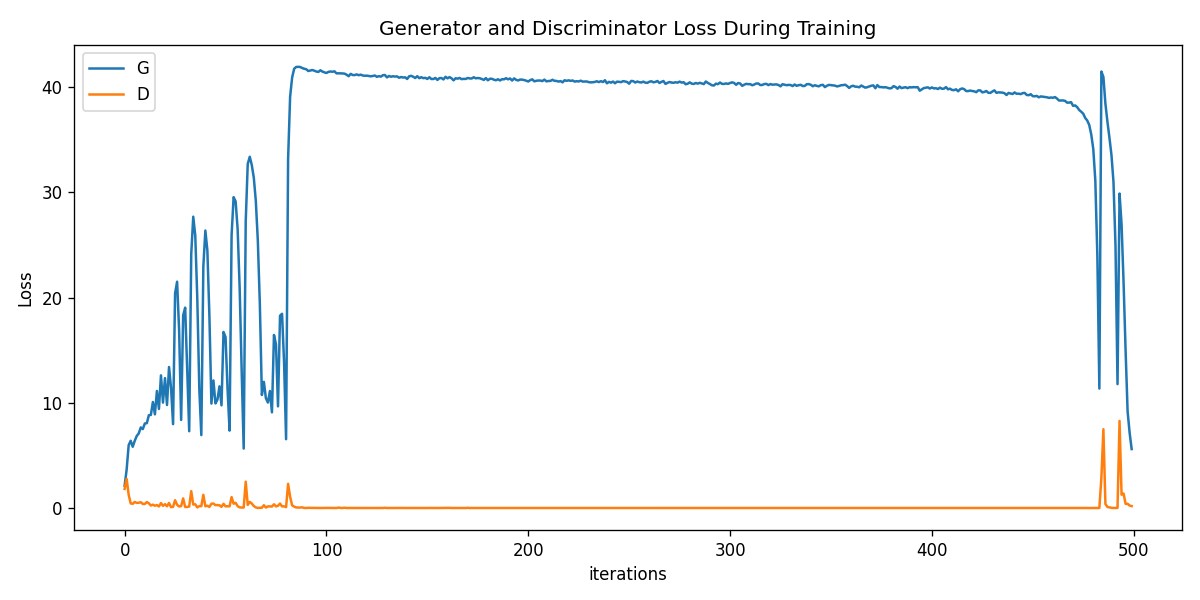
\includegraphics[width=0.88\textwidth]{runs/tutorial/loss_curve.png}}{Experiment 1. Generator and discriminator loss.}

\fixedfig{%
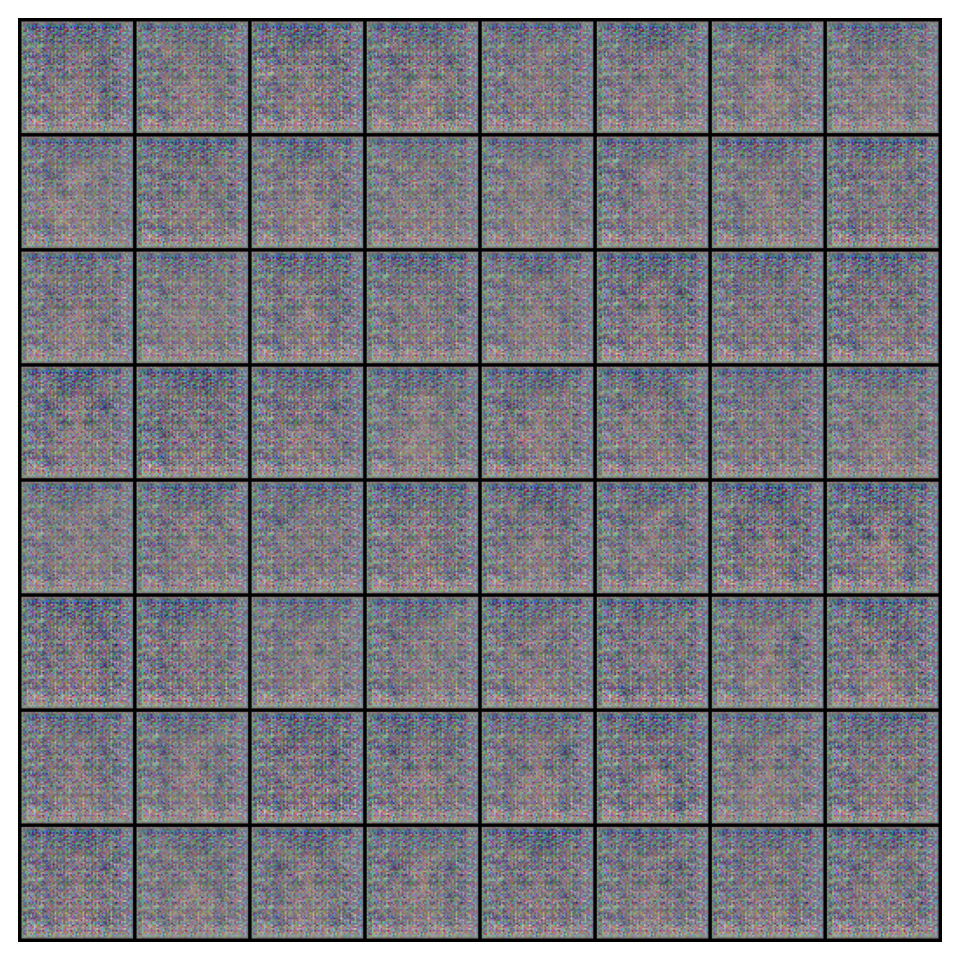
\includegraphics[width=0.18\textwidth]{runs/tutorial/epoch_1.png}\hfill
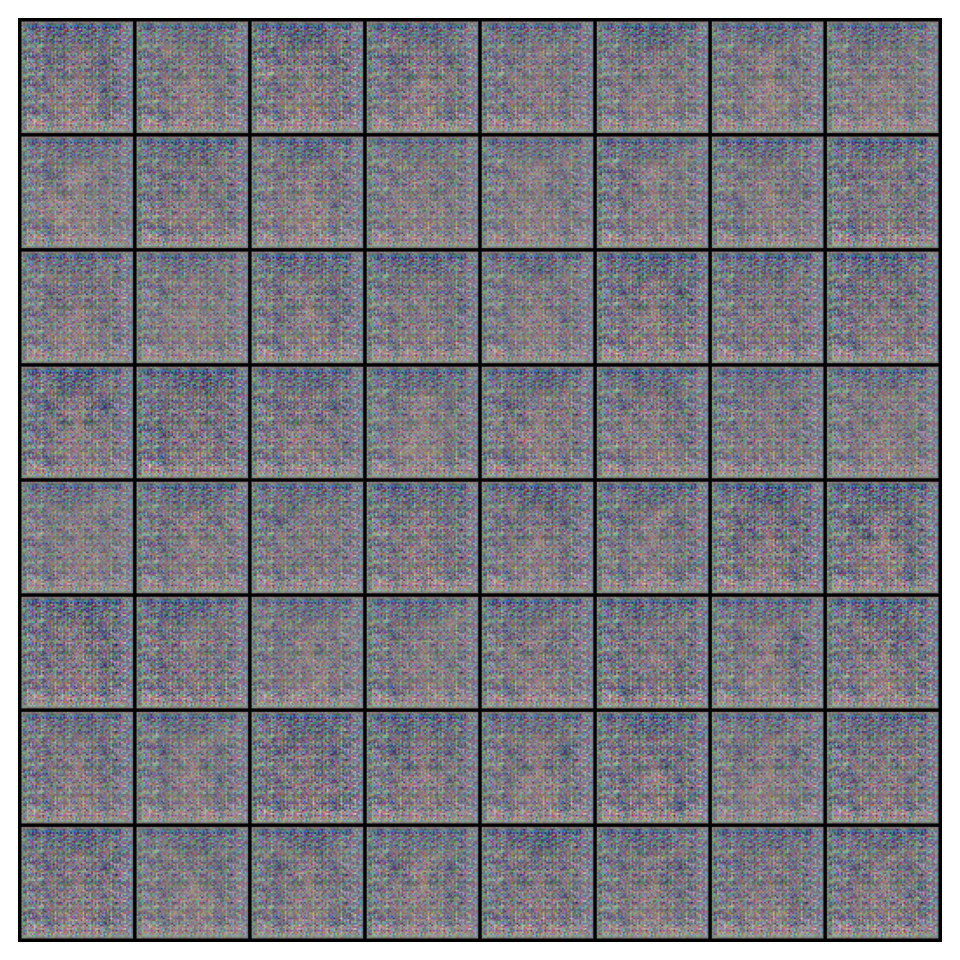
\includegraphics[width=0.18\textwidth]{runs/tutorial/epoch_2.png}\hfill
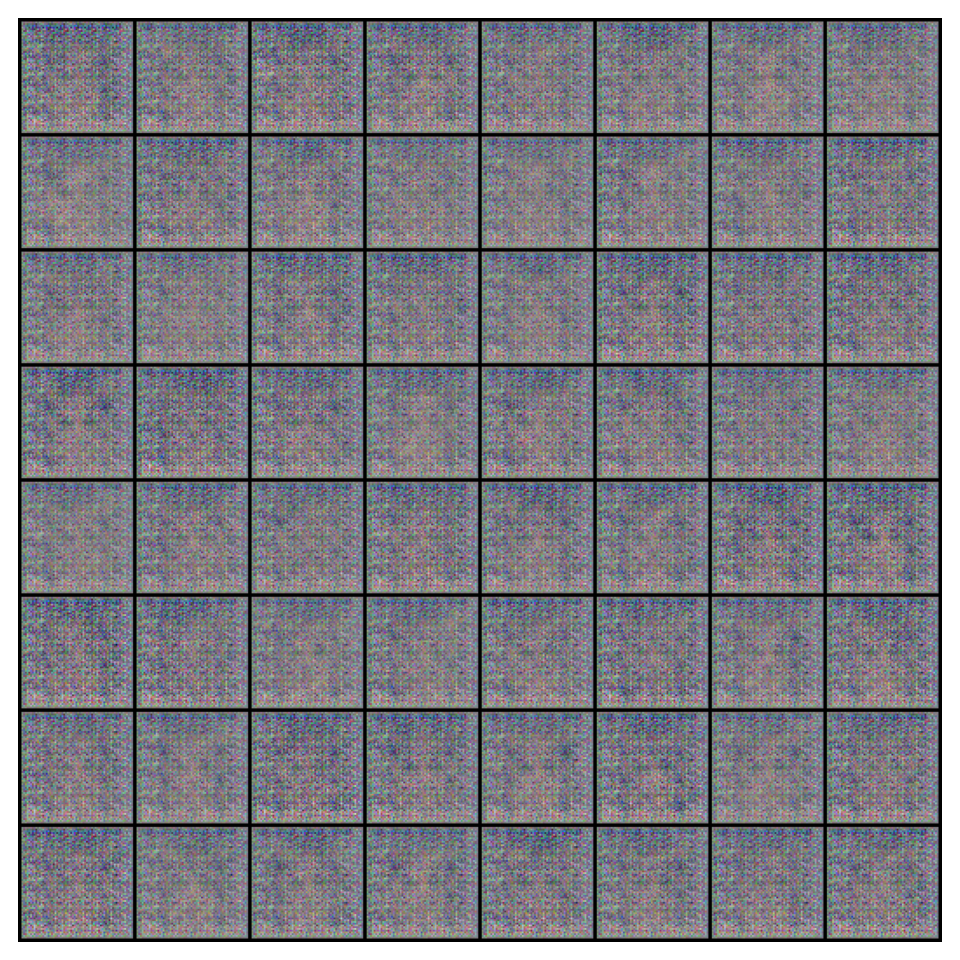
\includegraphics[width=0.18\textwidth]{runs/tutorial/epoch_3.png}\hfill
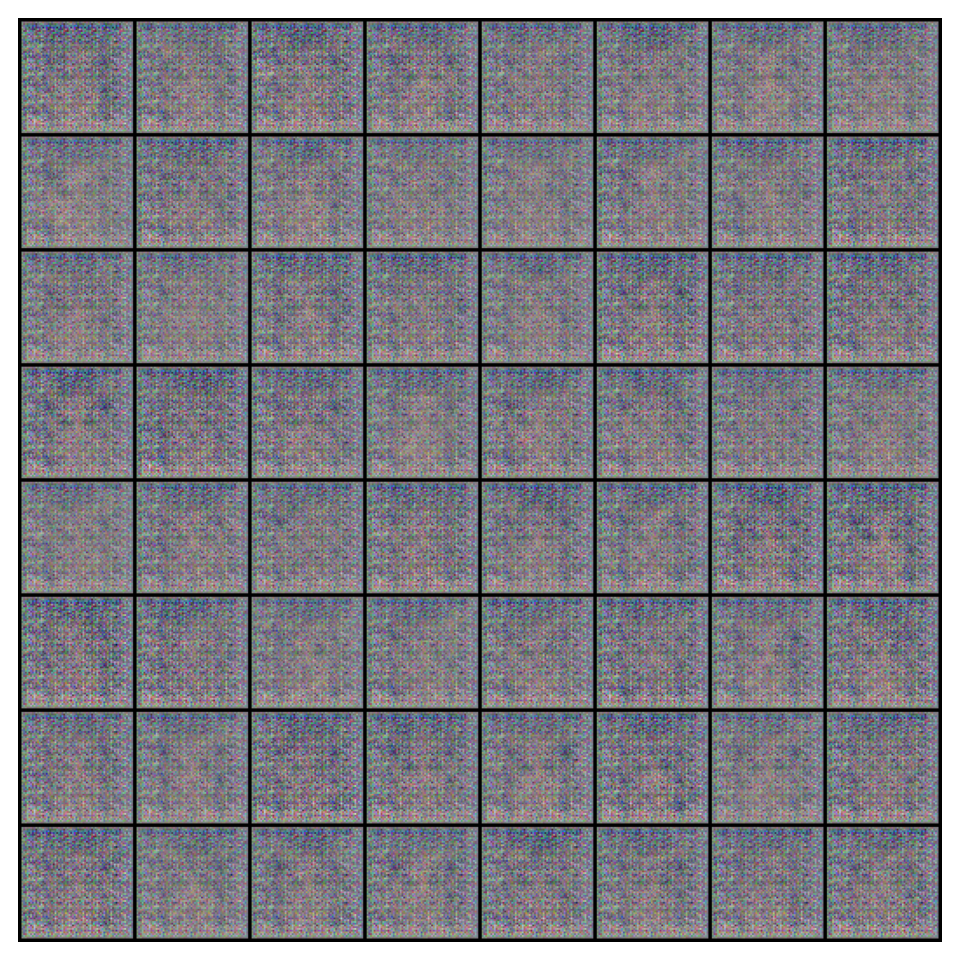
\includegraphics[width=0.18\textwidth]{runs/tutorial/epoch_4.png}\hfill
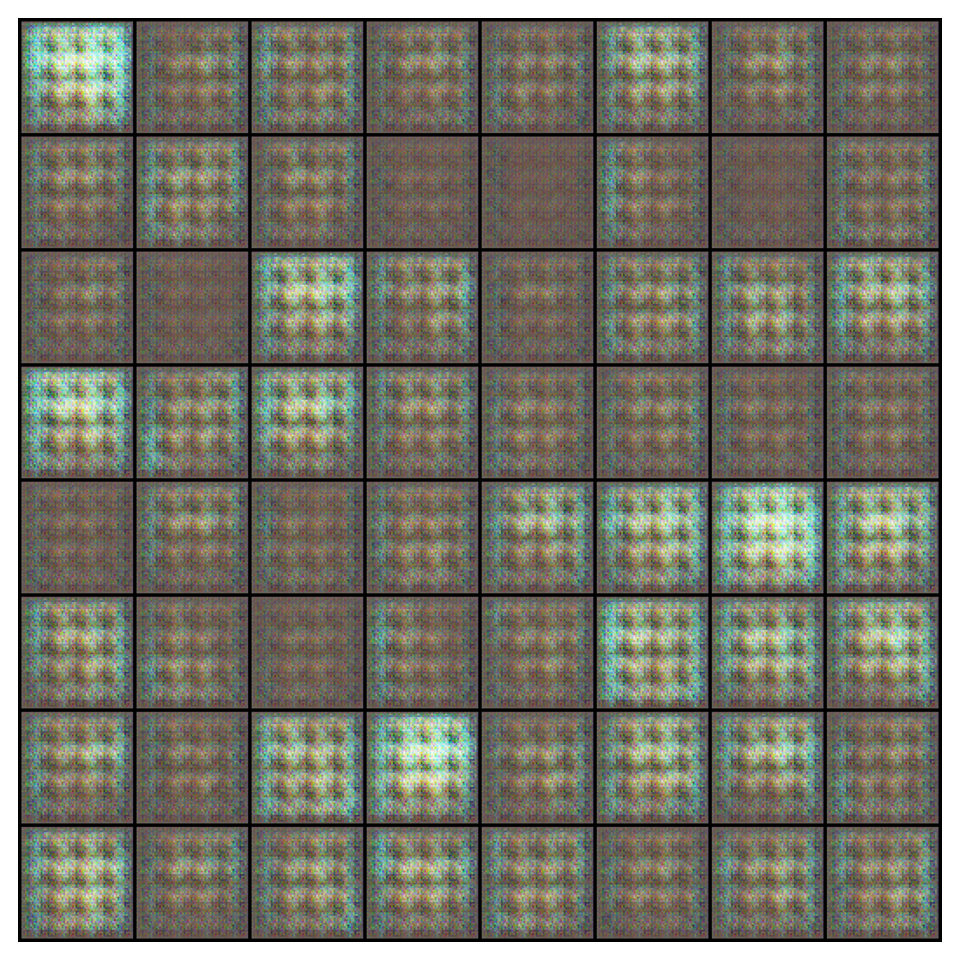
\includegraphics[width=0.18\textwidth]{runs/tutorial/epoch_5.png}%
}{Experiment 1. Fixed-noise outputs after epochs 1 through 5.}

\fixedfig{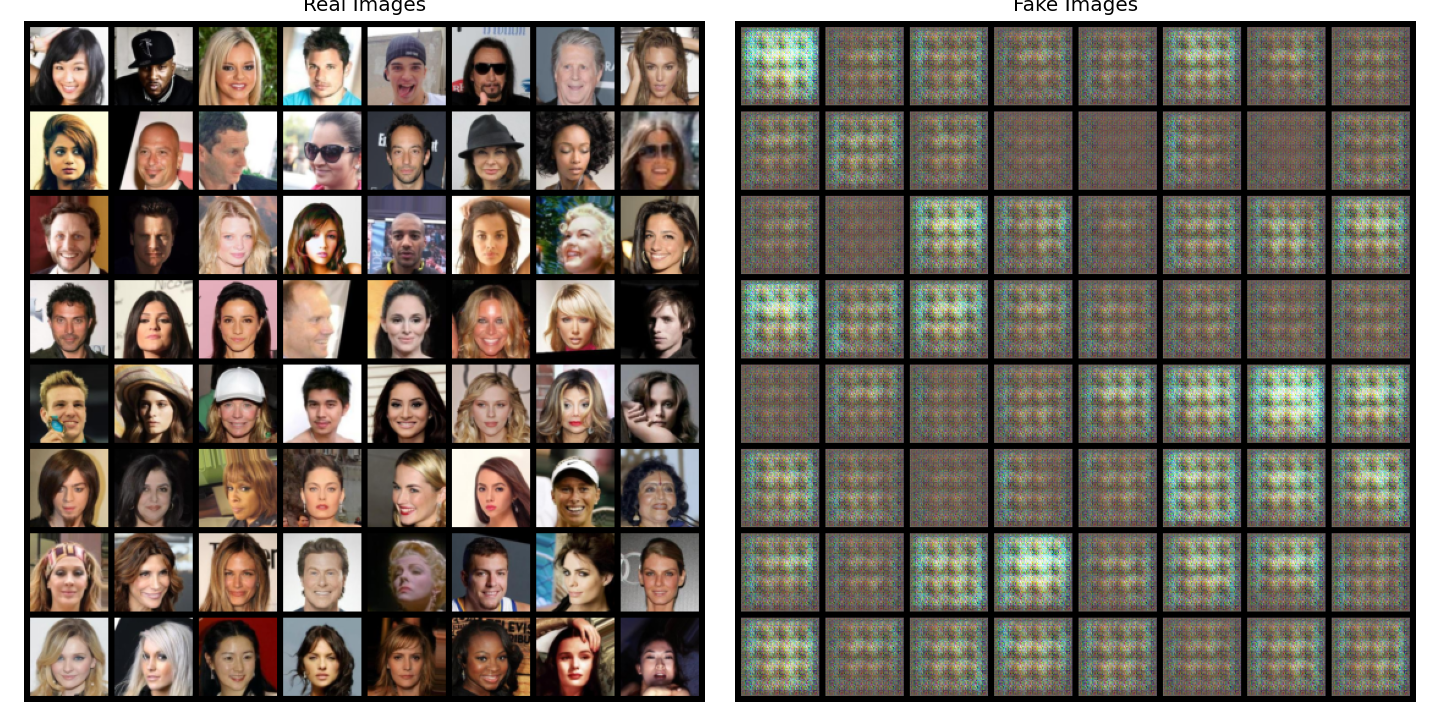
\includegraphics[width=0.88\textwidth]{runs/tutorial/real_vs_fake.png}}{Experiment 1. Real training images and the final generator samples.}

\section{Batch normalization}

Batch norm is applied to a convolution's output before the nonlinearity. For each channel it subtracts the minibatch mean, divides by the minibatch standard deviation, then applies a learned scale and shift.

In the generator it is on every conv-transpose layer except the last. Those layers turn the noise vector into a spatial feature map. A discriminator step changes what the generator has to match, so the activations inside the generator would otherwise jump and the next layer would see a new input distribution. Batch norm holds each feature map to a common scale, which is what lets both networks train at the DCGAN learning rate of 0.0002. The last layer is left without it because that layer is a tanh whose job is to put pixels in the range \(-1\) to \(1\). Normalizing that output would fight the image range.

In the discriminator, batch norm is only on the middle convolutions. The first layer has none, so the discriminator scores the image values themselves. The last convolution has none, so the sigmoid receives a raw score instead of a score forced back to zero mean. The middle layers keep the leaky ReLU features on a stable scale while the generator's outputs are moving. That matters because the discriminator's input distribution changes on every generator step. This is the DCGAN pattern: batch norm in both networks so gradients still reach the early layers, with those two layers left out.

The two-layer discriminator in experiment 3 is different on purpose. The assigned diagram puts batch norm after the first convolution, and that run follows the diagram.

\section{Experiment 2: discriminator updated five times as often}

The discriminator is updated on every batch. The generator is updated only when the iteration count is a multiple of 5, so there are five discriminator steps for each generator step. Each discriminator step uses a new real batch and a new noise sample. Over 5 epochs this is 500 discriminator updates and 100 generator updates.

\begin{verbatim}
d_repeat = 5
if iters % d_repeat == 0:
    update the generator to maximize log D(G(z))
\end{verbatim}

\begin{center}
\small
\begin{tabular}{@{}cccccc@{}}
\toprule
Epoch & Batch & Loss\(_D\) & Loss\(_G\) & \(D(x)\) & \(D(G(z))\) \\
\midrule
1 & 0 & 1.8134 & 2.1164 & 0.3093 & 0.3012 / 0.1568 \\
1 & 50 & 0.0274 & 18.7424 & 0.9818 & 0.0000 / 0.0000 \\
2 & 0 & 0.0044 & 20.4710 & 0.9959 & 0.0000 / 0.0000 \\
2 & 50 & 0.0012 & 34.5344 & 0.9988 & 0.0000 / 0.0000 \\
3 & 0 & 0.0001 & 13.6928 & 0.9999 & 0.0000 / 0.0000 \\
3 & 50 & 0.0005 & 39.0544 & 0.9995 & 0.0000 / 0.0000 \\
4 & 0 & 0.0000 & 39.0681 & 1.0000 & 0.0000 / 0.0000 \\
4 & 50 & 0.0001 & 39.1564 & 0.9999 & 0.0000 / 0.0000 \\
5 & 0 & 0.0000 & 38.9207 & 1.0000 & 0.0000 / 0.0000 \\
5 & 50 & 0.0001 & 39.1629 & 0.9999 & 0.0000 / 0.0000 \\
\bottomrule
\end{tabular}
\end{center}

\clearpage
Giving the discriminator more steps makes the imbalance worse, not better. It is confident by batch 50 of epoch 1, and it stays there. The generator loss ends near 39. The fixed-noise images remain noise. The assignment allows this: the schedule does not have to beat the baseline.

On the loss plot the generator curve is drawn only on the steps where the generator is updated, so it has one fifth as many points as the discriminator curve.

\fixedfig{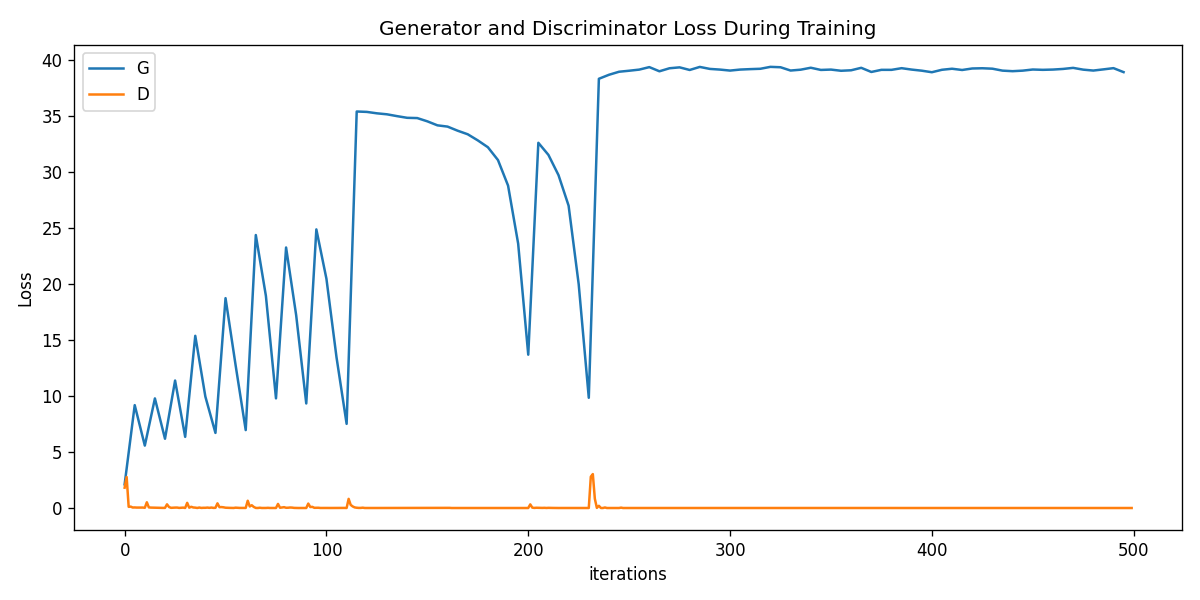
\includegraphics[width=0.88\textwidth]{runs/d5/loss_curve.png}}{Experiment 2. Generator and discriminator loss. The generator is updated every fifth step.}

\fixedfig{%
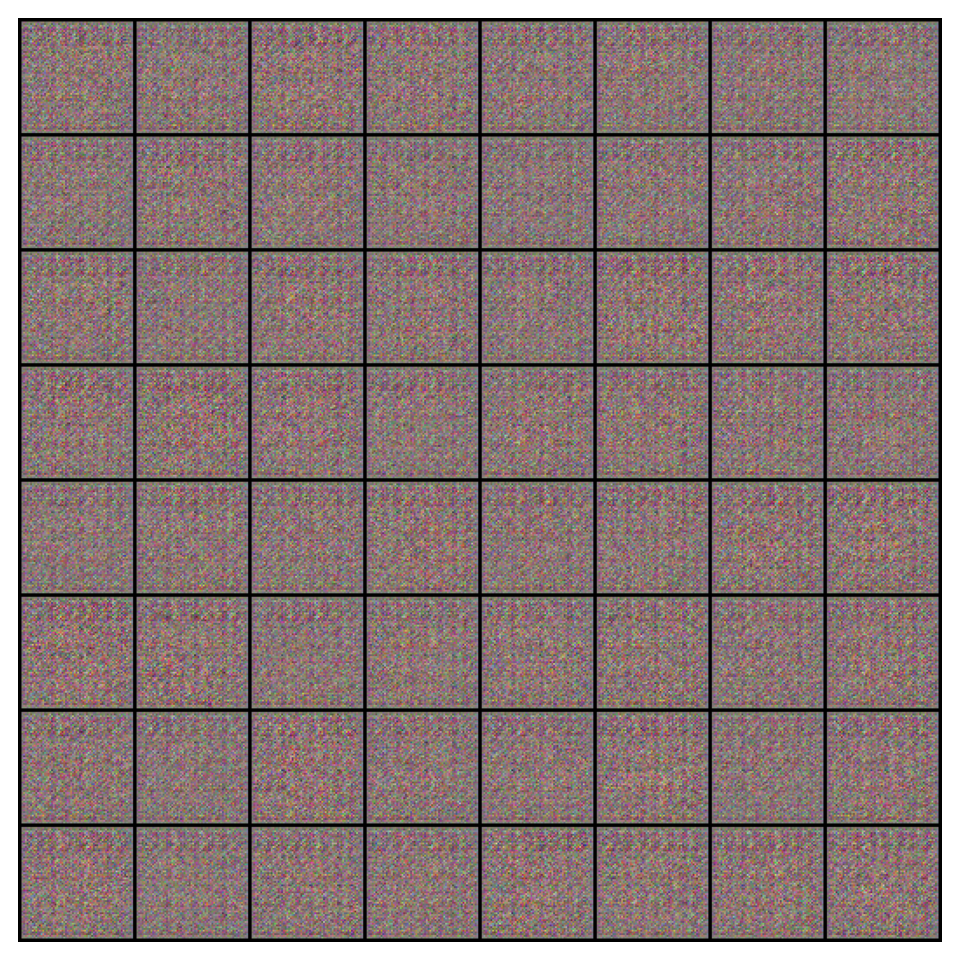
\includegraphics[width=0.18\textwidth]{runs/d5/epoch_1.png}\hfill
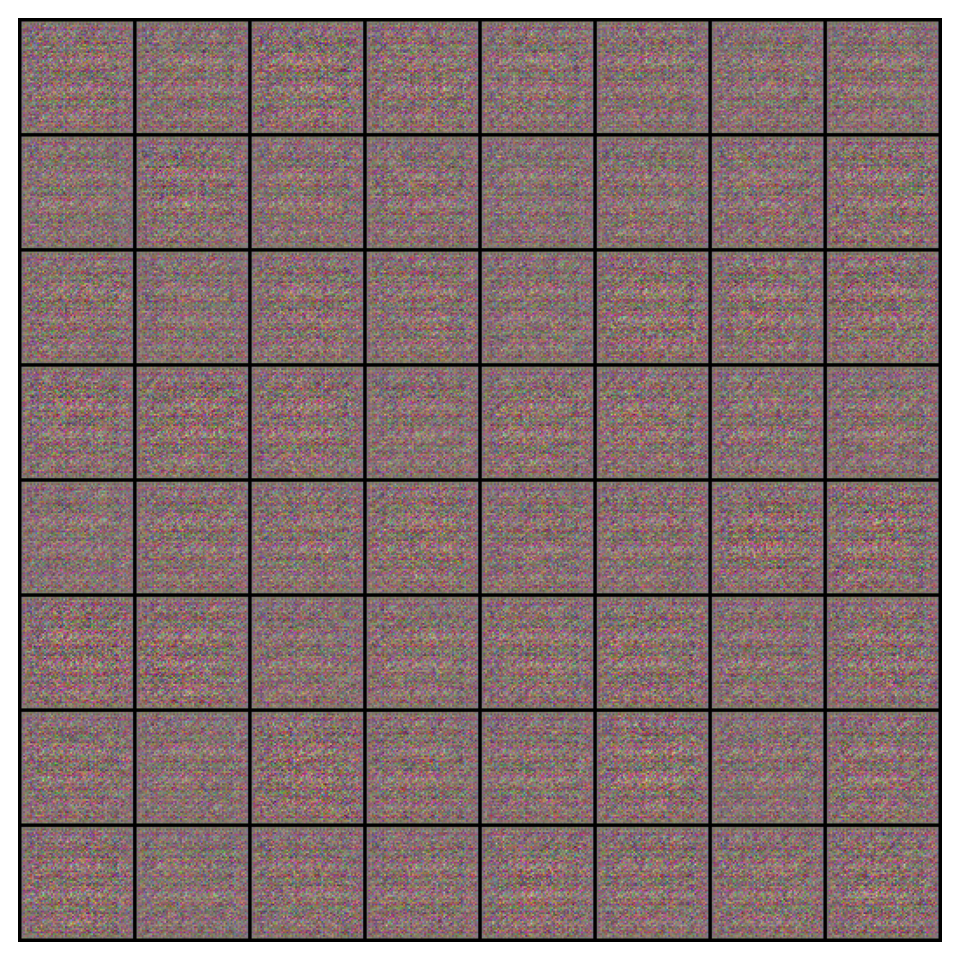
\includegraphics[width=0.18\textwidth]{runs/d5/epoch_2.png}\hfill
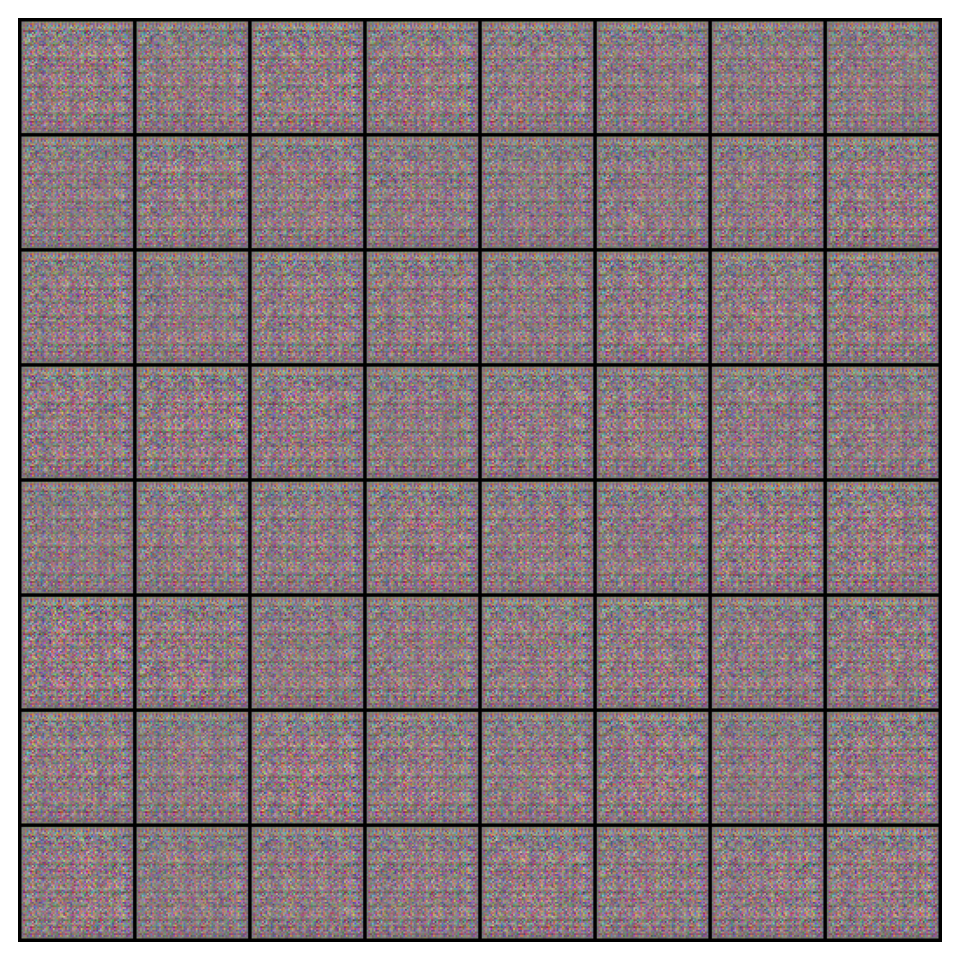
\includegraphics[width=0.18\textwidth]{runs/d5/epoch_3.png}\hfill
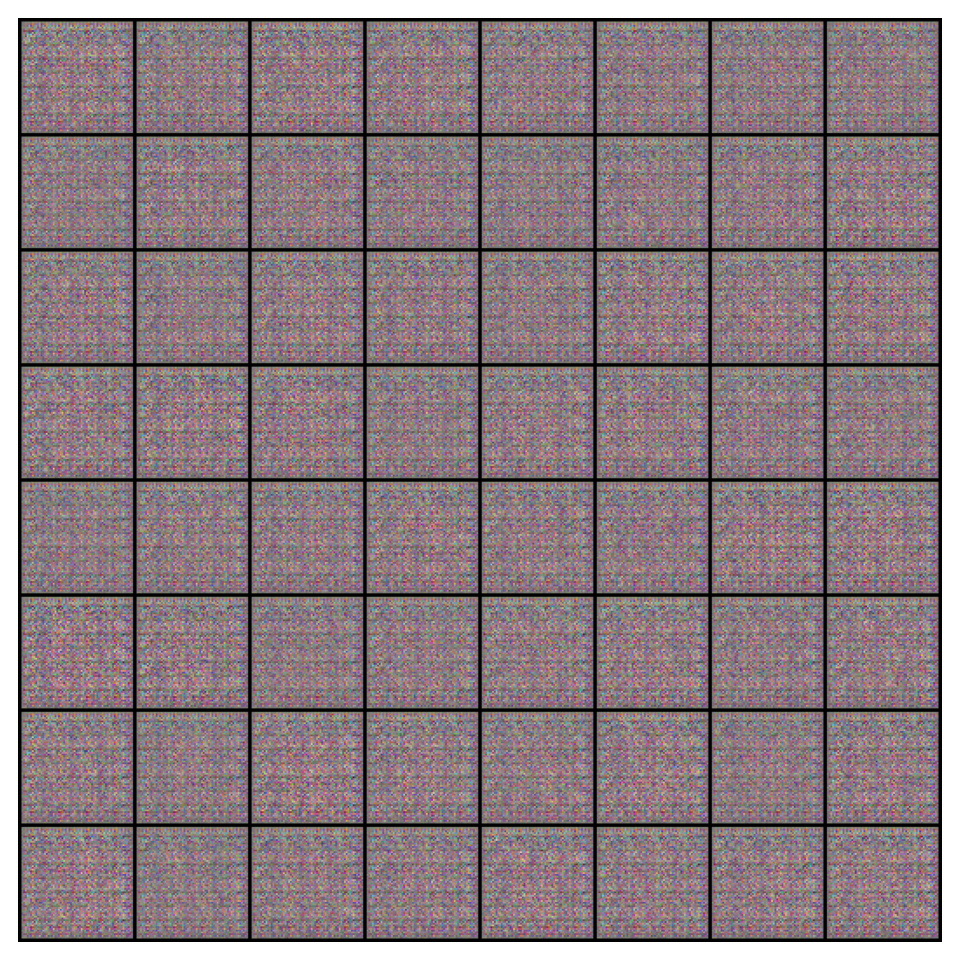
\includegraphics[width=0.18\textwidth]{runs/d5/epoch_4.png}\hfill
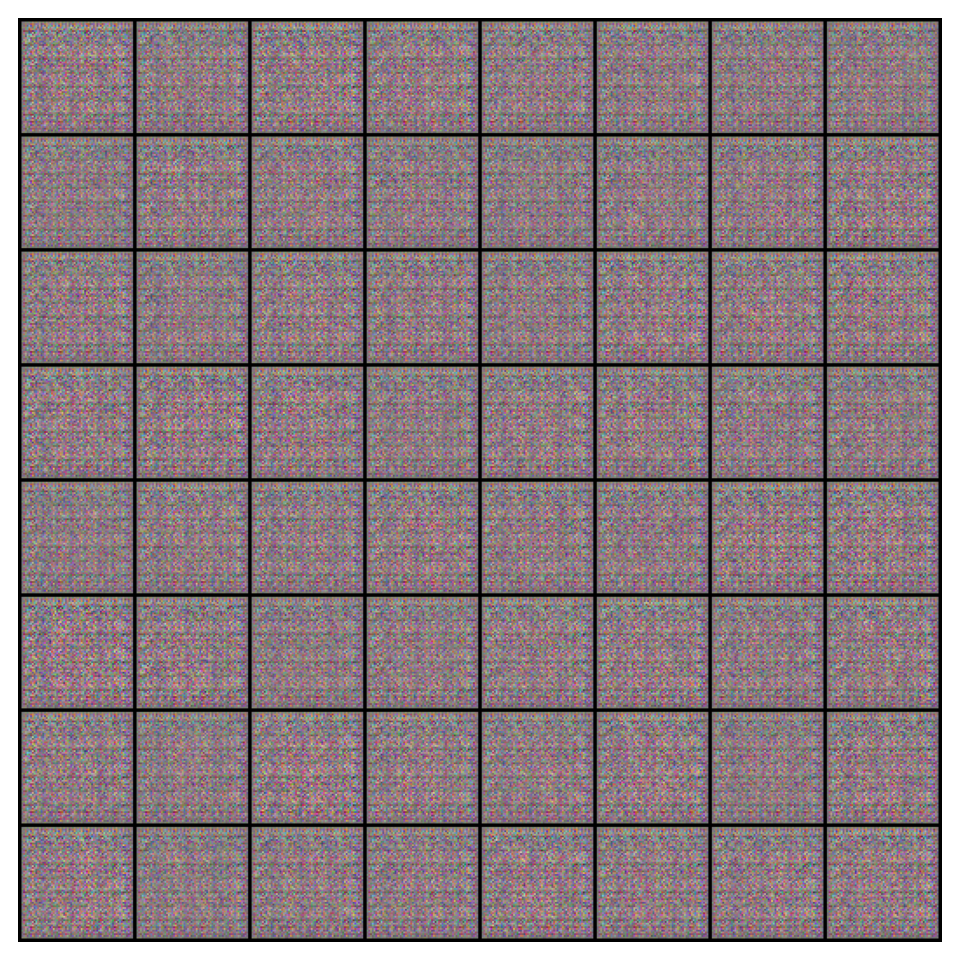
\includegraphics[width=0.18\textwidth]{runs/d5/epoch_5.png}%
}{Experiment 2. Fixed-noise outputs after epochs 1 through 5.}

\fixedfig{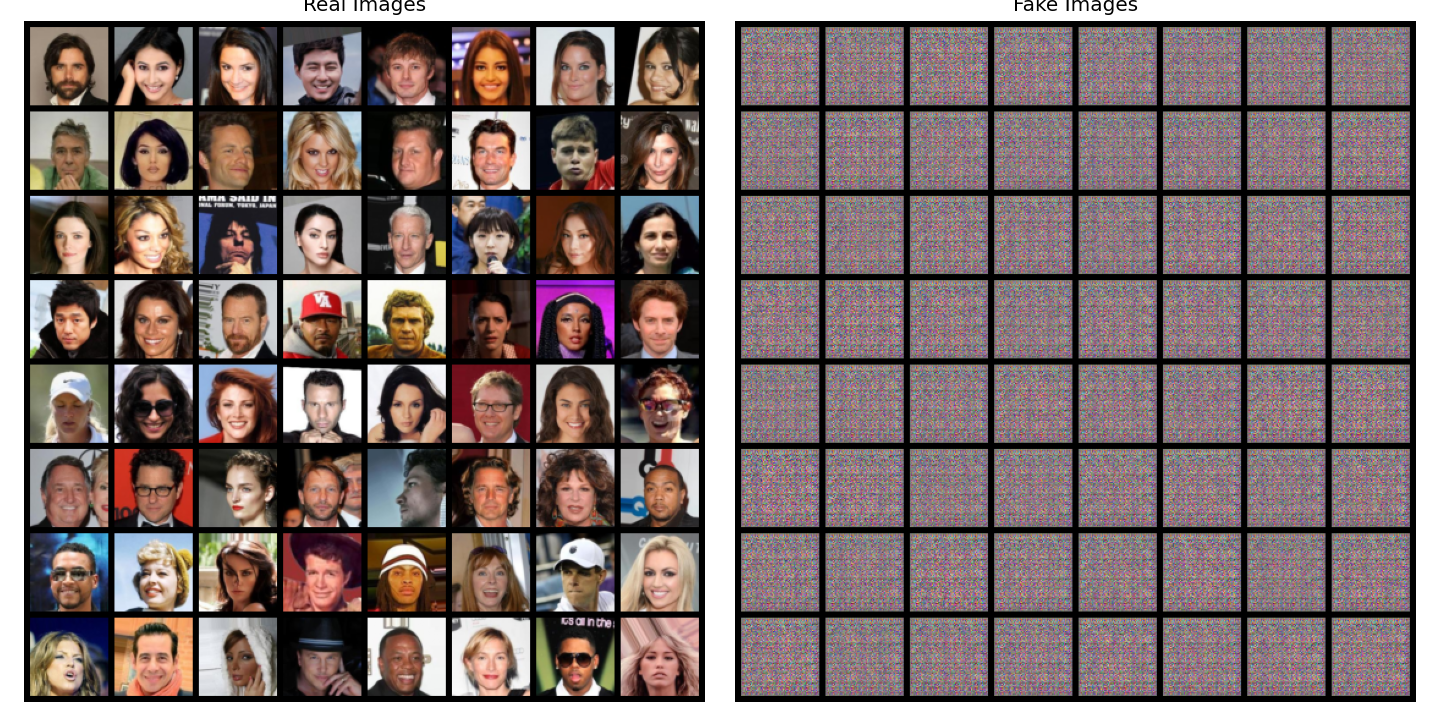
\includegraphics[width=0.88\textwidth]{runs/d5/real_vs_fake.png}}{Experiment 2. Real training images and the final generator samples.}

\clearpage
\section{Experiment 3: two-convolution discriminator}

The generator is unchanged and both networks start from new weights. The discriminator is the two-layer network from the assignment. The first convolution maps 3 channels to 64 with stride 2, then batch norm and a leaky ReLU. The second convolution maps 64 channels to 1 with stride 1 and no padding. Adaptive average pooling reduces that map to \(1\times 1\), and a sigmoid turns it into a probability. Training is back to one discriminator step per generator step.

\begin{verbatim}
Conv2d(3, 64, kernel_size=4, stride=2, padding=1, bias=False)
BatchNorm2d(64)
LeakyReLU(0.2, inplace=True)
Conv2d(64, 1, kernel_size=4, stride=1, bias=False)
AdaptiveAvgPool2d((1, 1))
Sigmoid()
\end{verbatim}

\begin{center}
\small
\begin{tabular}{@{}cccccc@{}}
\toprule
Epoch & Batch & Loss\(_D\) & Loss\(_G\) & \(D(x)\) & \(D(G(z))\) \\
\midrule
1 & 0 & 1.4062 & 0.6395 & 0.5338 & 0.5407 / 0.5275 \\
1 & 50 & 1.4150 & 0.6362 & 0.5195 & 0.5320 / 0.5293 \\
2 & 0 & 1.4166 & 0.6244 & 0.5240 & 0.5369 / 0.5356 \\
2 & 50 & 1.3937 & 0.6378 & 0.5277 & 0.5295 / 0.5285 \\
3 & 0 & 1.3795 & 0.6620 & 0.5219 & 0.5171 / 0.5158 \\
3 & 50 & 1.3628 & 0.6833 & 0.5200 & 0.5068 / 0.5050 \\
4 & 0 & 1.3484 & 0.7021 & 0.5203 & 0.4979 / 0.4955 \\
4 & 50 & 1.3299 & 0.7280 & 0.5203 & 0.4891 / 0.4829 \\
5 & 0 & 1.3059 & 0.7528 & 0.5244 & 0.4801 / 0.4710 \\
5 & 50 & 1.3122 & 0.7461 & 0.5193 & 0.4756 / 0.4742 \\
\bottomrule
\end{tabular}
\end{center}

This discriminator is too weak to separate real images from fakes. \(D(x)\) and \(D(G(z))\) both stay near \(0.5\) for all 5 epochs, so the generator is never pushed to match a face. Its samples pick up a repeated color pattern, not a person. The losses do stay finite and move slowly: discriminator loss ends at 1.30 and generator loss at 0.76. That is a stable failure, unlike the saturated baseline.

\fixedfig{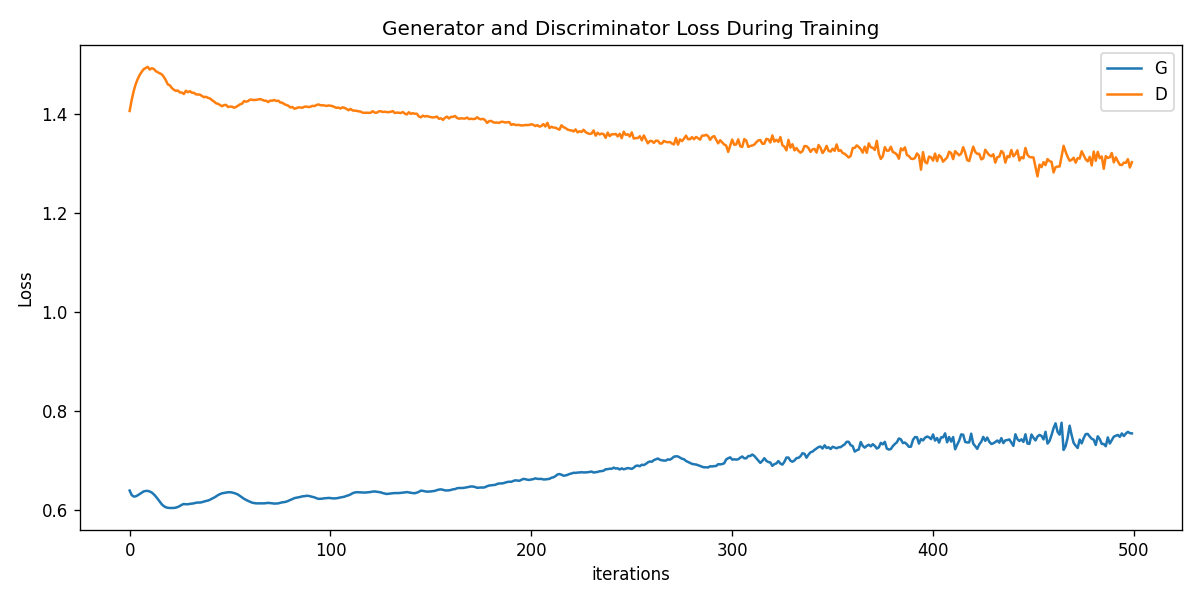
\includegraphics[width=0.88\textwidth]{runs/simple/loss_curve.png}}{Experiment 3. Generator and discriminator loss.}

\fixedfig{%
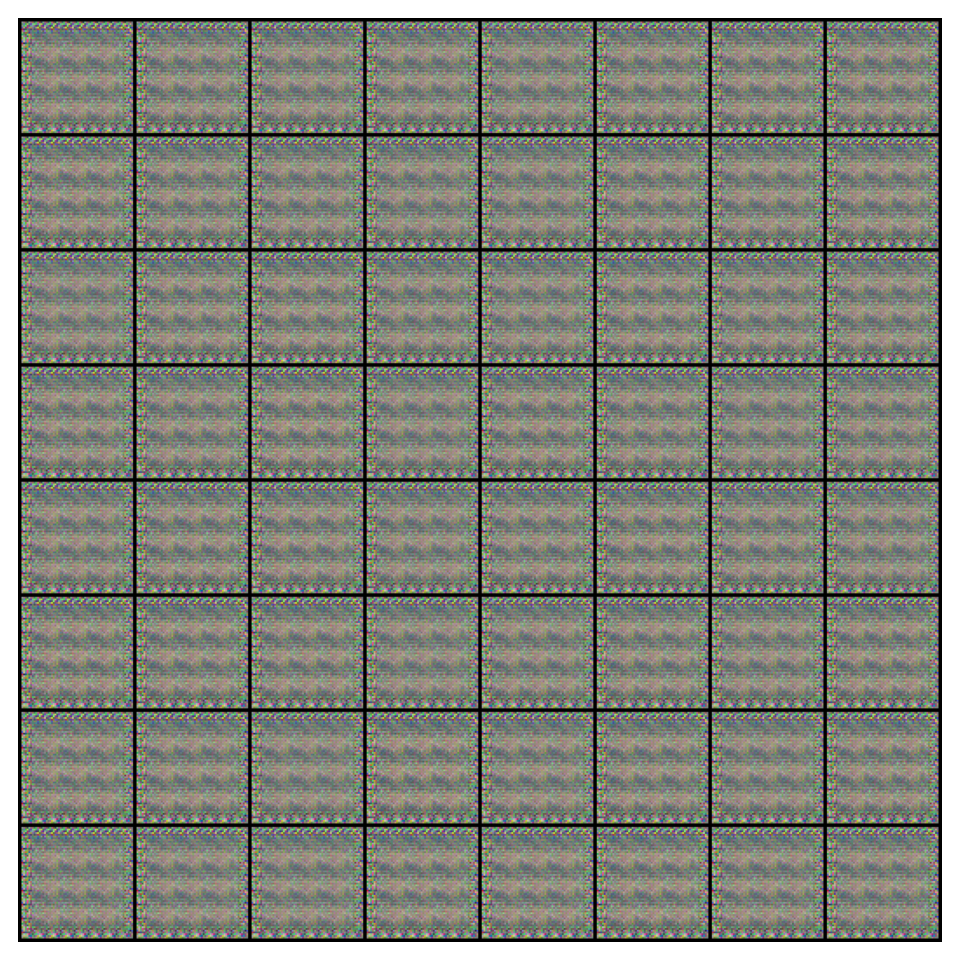
\includegraphics[width=0.18\textwidth]{runs/simple/epoch_1.png}\hfill
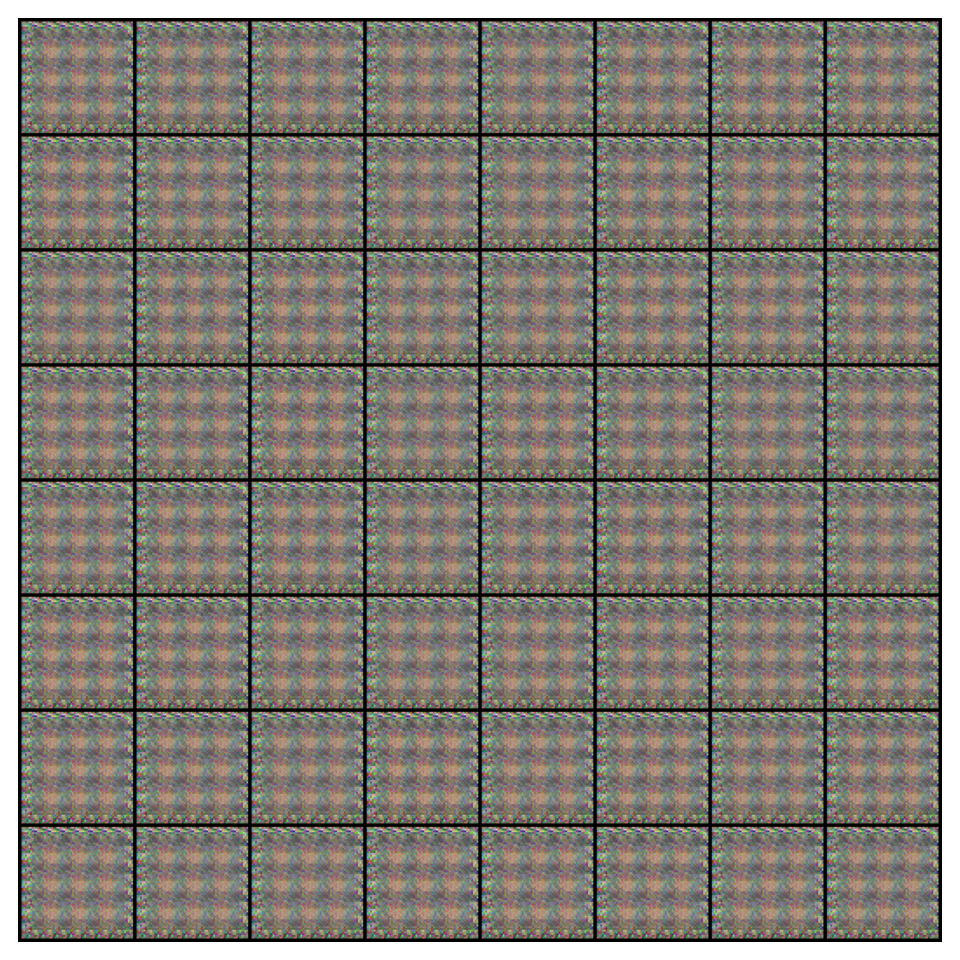
\includegraphics[width=0.18\textwidth]{runs/simple/epoch_2.png}\hfill
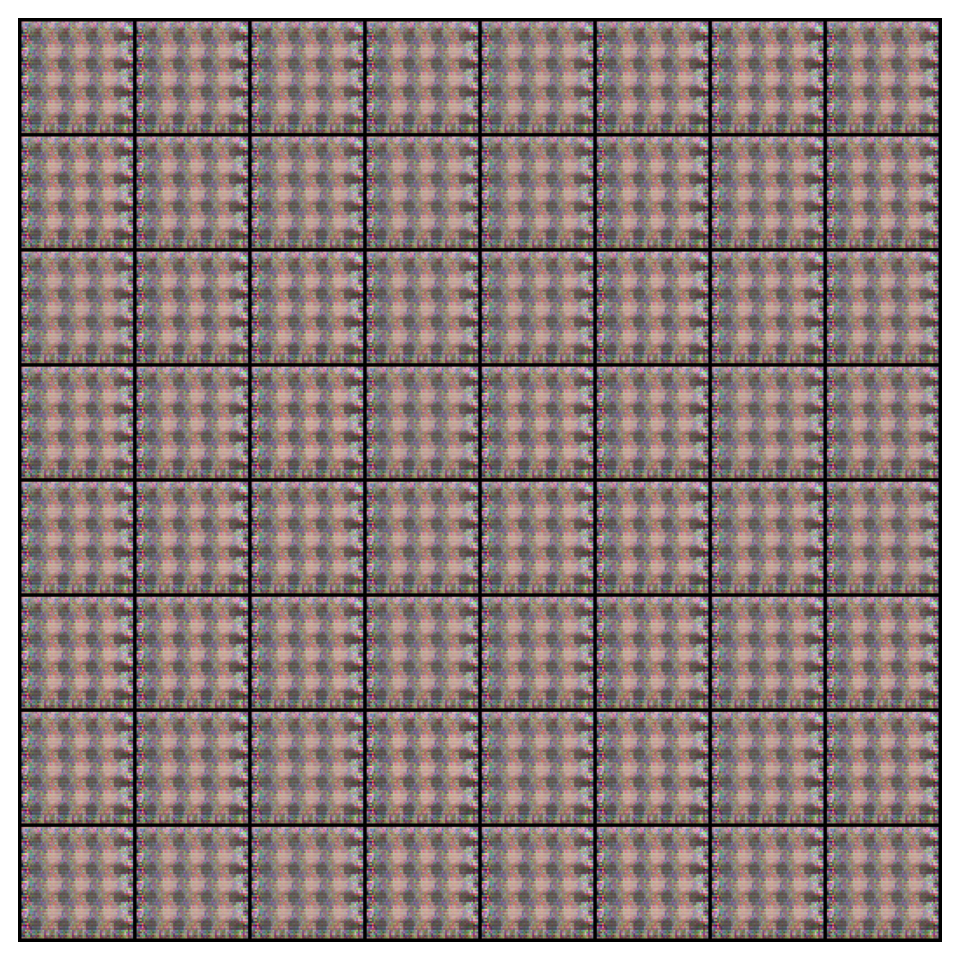
\includegraphics[width=0.18\textwidth]{runs/simple/epoch_3.png}\hfill
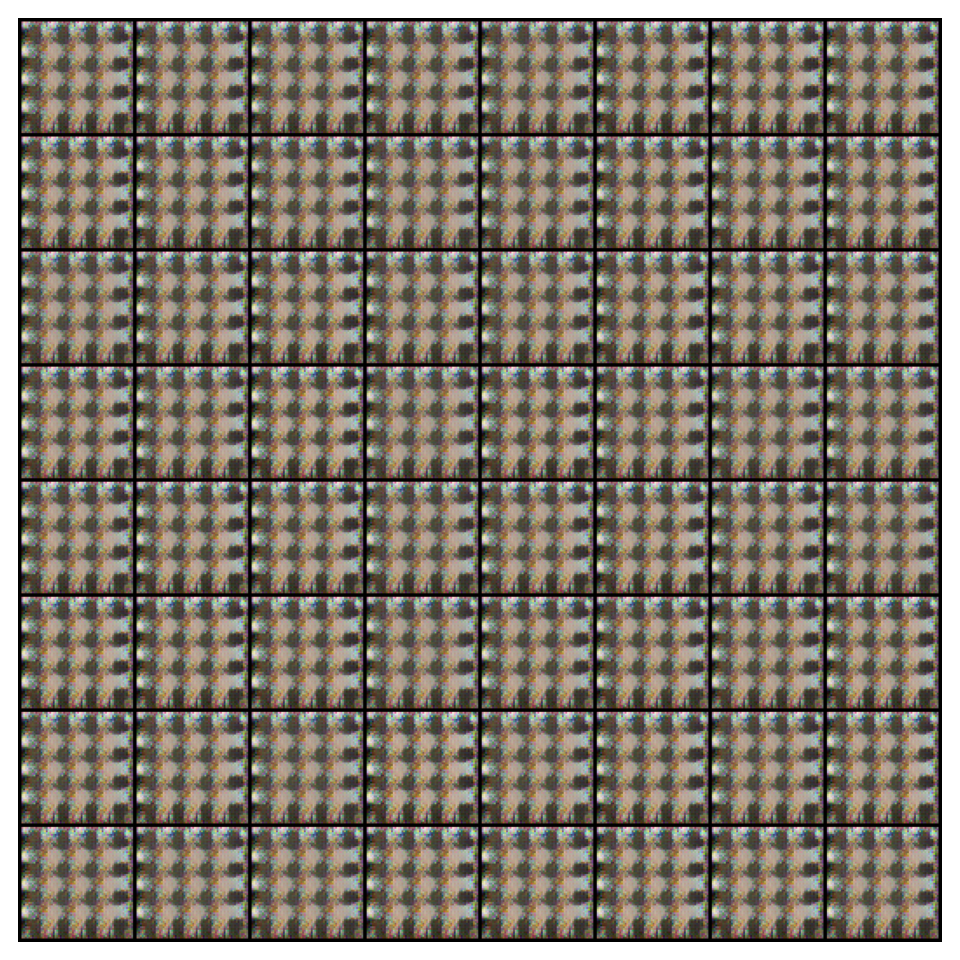
\includegraphics[width=0.18\textwidth]{runs/simple/epoch_4.png}\hfill
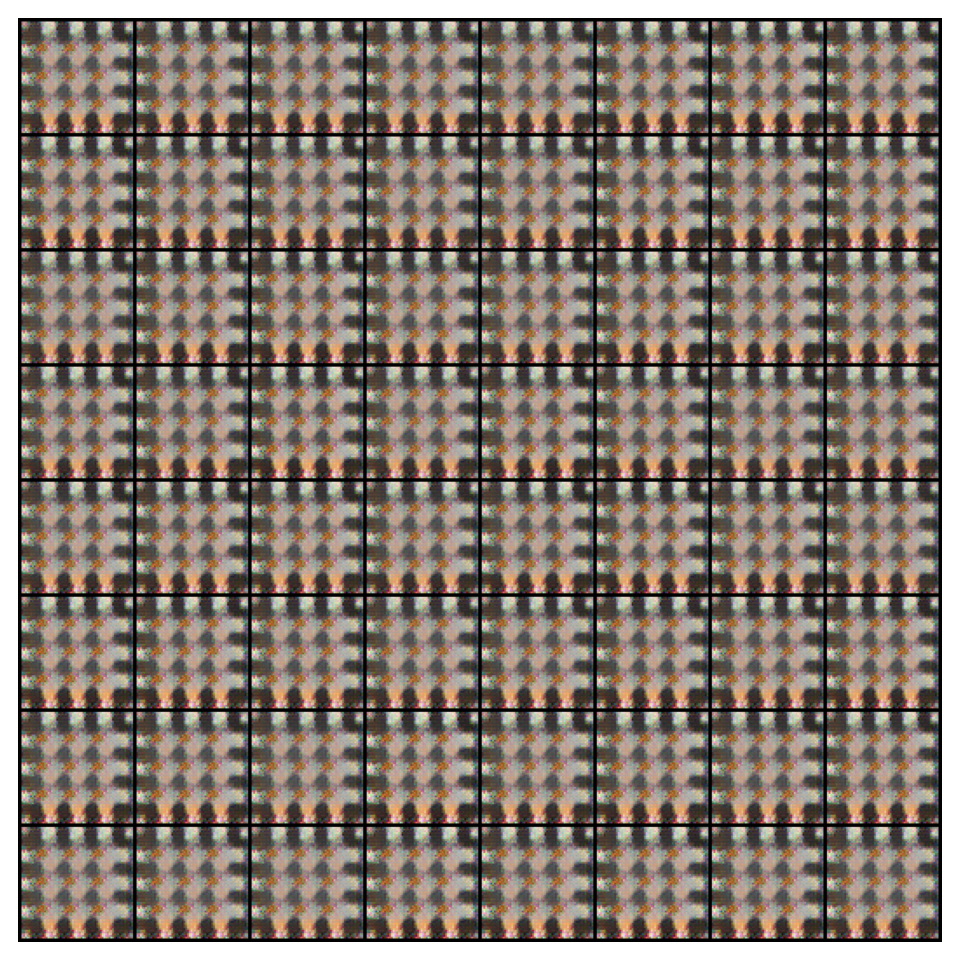
\includegraphics[width=0.18\textwidth]{runs/simple/epoch_5.png}%
}{Experiment 3. Fixed-noise outputs after epochs 1 through 5.}

\fixedfig{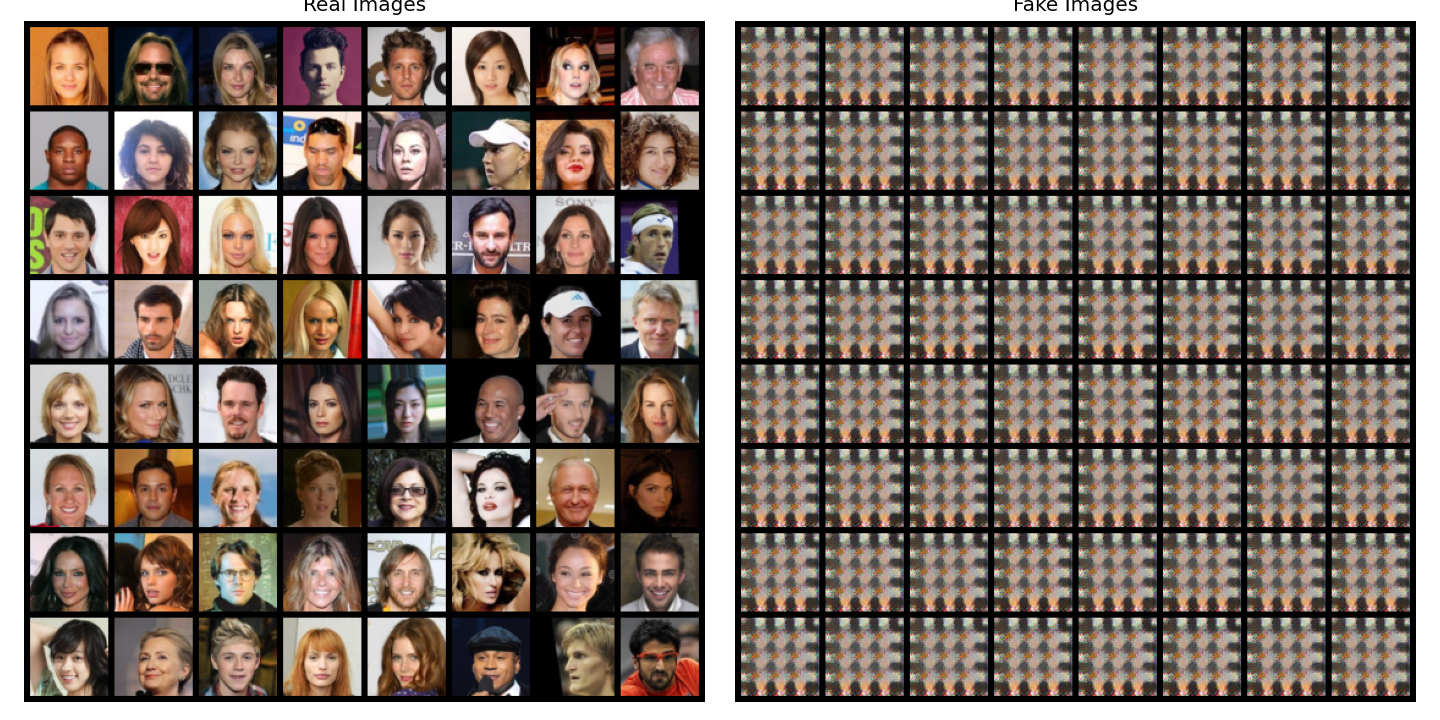
\includegraphics[width=0.88\textwidth]{runs/simple/real_vs_fake.png}}{Experiment 3. Real training images and the final generator samples.}

\end{document}
